\documentclass{beamer}
\usetheme{default}
\useoutertheme{miniframes}
\useinnertheme{circles}
\usepackage{graphicx}
\usepackage{hyperref}
\usepackage{pdfpages}
\usepackage{pgf}  
\logo{\pgfputat{\pgfxy(-11, 0)}{\pgfbox[center,base]{
\includegraphics[width=2.5cm]{ANUlogo.png}}}} 

\definecolor{ANUbg}{rgb}{0.2, 0.2, 0.2}
\definecolor{ANUblue}{rgb}{0.56, 0.69, 0.75}
\usecolortheme[named=ANUbg]{structure}

\title{Machine Learning Approaches to Computational Protein Design}


\author{Stephen Zhang}

% Let's get started
\begin{document}

\begin{frame}
  \titlepage
\end{frame}

\section{Introduction}

\begin{frame}
    \begin{itemize}
        \item Computational techniques can be used to design mutant aaRS that exhibit affinity and specificity for corresponding uAAs.
        \item Major utility of computational protein design - \textit{huge reduction of search space}
        \item \texttt{Rosetta} is a state-of-the-art software package for a wide range of protein computation protocols.
    \end{itemize}
\end{frame}

\begin{frame}
    Conventional workflow is as follows...
    \begin{enumerate}
        \item Construct protein model (e.g. \textit{Mj}TyrRS, pCNFRS) based off crystal structures. Place uAA in binding site, specify mutation sites and kinetic constraints.
        \item Generate mutant candidates using \texttt{Rosetta} protocols. Calculate various score factors for mutants.
        \begin{center}Mutant pose $\to$ $\mathrm{scores}(E_1, E_2, E_3, ...)$\end{center}
        \item Select candidates for \textit{in vitro} experimentation by applying thresholds or ranking w.r.t several score factors (e.g. total score, ligand binding score), e.g. $\underbrace{\text{total score} > E_0}_{\text{a rectangular constraint!}}$
    \end{enumerate}
\end{frame}

\begin{frame}
    This has significant limitations: boundary between 'good' and 'bad' may be nonlinear! \\
    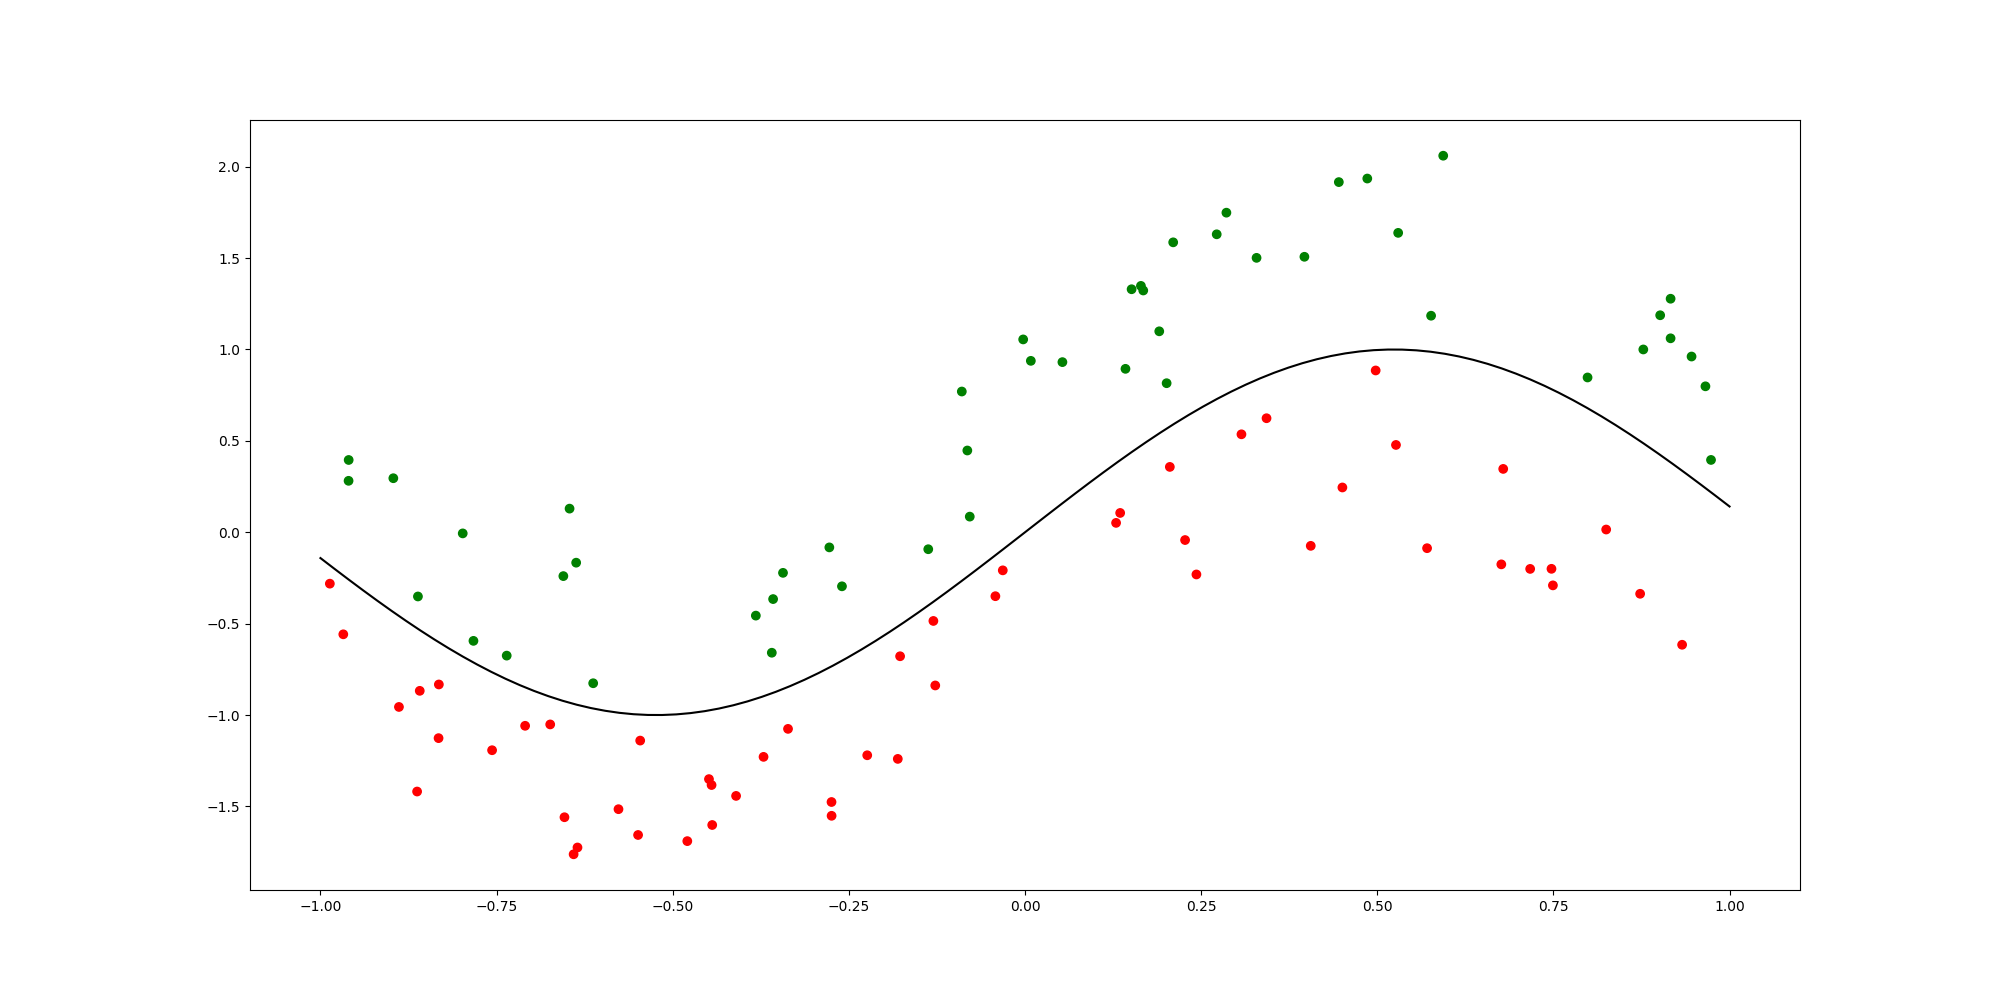
\includegraphics[width=\linewidth]{diagram2.png}
\end{frame}

\begin{frame}
    Machine learning techniques, specifically \textbf{binary classifiers}, can be used to deal with these situations.
\begin{enumerate}
\item For each candidate protein, we have a set of \texttt{Rosetta} scores \texttt{fa\_atr}, \texttt{fa\_sol}, ...
    These are called \textbf{factors}. Any candidate mutant is described by a vector of factors in a high-dimensional space:
    $$\vec{x} = (E_1, E_2, E_3, ..., E_m)$$
    
    \item Each candidate mutant is associated with its \textbf{class} $\in \{0, 1\}$. Here, 0 = 'non binding', 1 = 'binding'. We seek a map $F : \vec{x} \in \mathbb{R}^m \to \{0, 1\}$ that can predict \textbf{class} from \textbf{factors}.
    
    \item Machine learning methods allow approximations for such a function $F$ to be iteratively \textbf{learned} by a computer.
\end{enumerate}
\end{frame}

\begin{frame}
    Three binary classification approaches were employed, implemented in Python using \texttt{sklearn} library.
    \begin{enumerate}
        \item Logistic regression | linear model
    \item Artificial neural network (ANN) | nonlinear model
        \item Support vector machine (SVM) | nonlinear model
    \end{enumerate}
\end{frame}

\section{Methods}
\begin{frame}{Training set}
    Training set comprised of uAAs reported in a literature review to be incorporated by \textit{p}CNFRS mutant.
    
    Dumas et al., \textit{Chem. Sci.}, 2015, 6, 50 $\rightarrow$ 60 mutant-uAA pairs.
    
    uAA ligands were \textbf{chemically diverse.}
    
    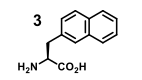
\includegraphics[scale = 0.4]{uAA3.png}
    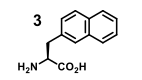
\includegraphics[scale = 0.4]{uAA5.png}
    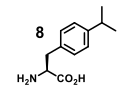
\includegraphics[scale = 0.4]{uAA8.png}
    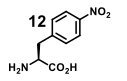
\includegraphics[scale = 0.4]{uAA12.png}
    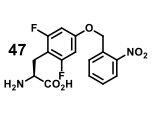
\includegraphics[scale = 0.4]{uAA47.png}
\end{frame}

\begin{frame}{Methods}
    \begin{itemize}
        \item Molecular models of uAA ligands constructed, 200 conformers generated using \texttt{balloon}
        \item Mutations modelled onto sequence of \textit{p}CNFRS (PDBID \texttt{3QE4})
        \item uAAs placed in aaRS binding cavity of \textit{p}CNFRS crystal structure using \texttt{pymol}
        \item Catalytic constraints manually specified for each mutant-uAA pair
        \item 500 candidate protein poses generated for \textbf{each} mutant-uAA pair using Rosetta \texttt{EnzymeDesign}
    \end{itemize}
    \begin{center}$\Rightarrow$ $(+)$ dataset!\end{center}
\end{frame}

\begin{frame}{Methods}
    For binary classification, using a \textbf{balanced} training dataset is important to avoid bias. Previous protocol repeated to produce the following datasets:
    \begin{itemize}
        \item Mutants against uAAs $(+)$
        \item Mutants against Tyr $(-)$
    \end{itemize}
    \begin{itemize}
        \item Wt \textit{Mj}TyrRS against uAAs $(-)$
        \item Wt \textit{Mj}TyrRS against Tyr $(+)$
    \end{itemize}
    
    Smaller datasets were randomly oversampled so that all four datasets were of equal size.
\end{frame}

\begin{frame}{Implementation}
    Machine learning algorithms were implemented in \texttt{python} using the \texttt{sklearn} library.
    \begin{itemize}
        \item $k$-fold cross-validation is standard practice to measure classifier accuracy. Here $k = 5$
        \item Points were grouped with respect to mutant-uAA pair to prevent 'cheating'
        \item CV score reported as arithmetic mean of individual scores
        \item Parameter optimisation carried out using \textbf{grid search}
    \end{itemize}
\end{frame}

\begin{frame}
    Optimal parameters resulted in:
    \begin{itemize}
        \item Logistic regression: \texttt{C = 1e3}
        \item ANN: hidden layer: 2$\times$24 neurons,
    \end{itemize}
\end{frame}

\begin{frame}{Acknowledgements}
\begin{itemize}
    \item \textbf{Prof. Thomas Huber}
    \item Haocheng Qianzhu
    \item Abeera Saeed
    \item Youssef Latash
\end{itemize}


\end{frame}
\end{document}


